\documentclass{article}

% Language setting
% Replace `english' with e.g. `spanish' to change the document language
\usepackage[english]{babel}

% Set page size and margins
% Replace `letterpaper' with `a4paper' for UK/EU standard size
\usepackage[letterpaper,top=2cm,bottom=2cm,left=3cm,right=3cm,marginparwidth=1.75cm]{geometry}

% Useful packages
\usepackage{amsmath}
\usepackage{graphicx}
\usepackage[colorlinks=true, allcolors=blue]{hyperref}

\title{Analyzation and improvement of moucha.org}
\author{Denes Laszlo Fekete}

\usepackage[nonumberlist, acronym]{glossaries}
\newacronym{AAA}{AAA}{Authentication, Authorization, and Accounting}
\newacronym{AS}{AS}{Autonomous System}
\newacronym{AVGW}{AVGW}{Analog Voice Gateway}
\newacronym{BGP}{BGP}{Border Gateway Protocol}
\newacronym{CAPWAP}{CAPWAP}{Control and Provisioning of Wireless Access Point}
\newacronym{CUCM}{CUCM}{Cisco Unified Call Manager}
\newacronym{DGK}{DGK}{Directory Gatekeeper Service}
\newacronym{DHCP}{DHCP}{Dynamic Host Configuration Protocol}
\newacronym{DNAC}{DNA-C}{Digital Network Architecture Center}
\newacronym{DPI}{DPI}{Deep Packet Inspection}
\newacronym{DSP}{DSP}{Digital Signalling Processor}
\newacronym{DVGW}{DVGW}{Digital Voice Gateway}
\newacronym{eBGP}{eBGP}{Exterior Border Gateway Protocol}
\newacronym{EID}{EID}{End Device Identifier}
\newacronym{FBN}{FBN}{Fabric Border Node}
\newacronym{FCN}{FCN}{Fabric Control Node}
\newacronym{FEN}{FEN}{Fabric Edge Node}
\newacronym{FVWLC}{F(V)WLC}{Fabric (Virtual) Wireless Lan Controller}
\newacronym{FXS}{FXS}{Foreign Exchange Station}
\newacronym{GSM}{GSM}{Global System for Mobile communication}
\newacronym{GUI}{GUI}{Graphical User Interface}
\newacronym{iBGP}{iBGP}{ Interior Border Gateway Protocol}
\newacronym{IP}{IP}{Internet Protocol}
\newacronym{IPVGW}{IPVGW}{IP Voice Gateway}
\newacronym{ISDN}{ISDN}{Integrated Services Digital Network}
\newacronym{iSE}{iSE}{Identity Services Engine}
\newacronym{LAN}{LAN}{Local Area Network}
\newacronym{LAP}{LAP}{Lightweight Access Point}
\newacronym{LER}{LER}{Label Edge Router }
\newacronym{LISP}{LISP}{Locator ID Separation Protocol}
\newacronym{LSR}{LSR}{Label Switch Router}
\newacronym{MAC}{MAC}{Media Access Control}
\newacronym{MEC}{MEC}{MultiChassis Etherchannel}
\newacronym{MPLS}{MPLS}{Multiprotocol Label Switching}
\newacronym{PoE}{PoE}{Power over Ethernet}
\newacronym{POTS}{POTS}{Plain Old Telephone Service}
\newacronym{PRI}{PRI}{Primary Rate Interface}
\newacronym{PSTN}{PSTN}{Public Service Telephone Network}
\newacronym{QoE}{QoE}{Quality of Service}
\newacronym{RIB}{RIB}{Routing Information Base}
\newacronym{SDN}{SDN}{Software-Defined Network}
\newacronym{SD-A}{SD-A}{Software-Defined Access}
\newacronym{SD-WAN}{SD-WAN}{Software-Defined Wide Area Network}
\newacronym{SIP}{SIP}{Session Initiation Protocol}
\newacronym{TCP}{TCP}{Transmission Control Protocol}
\newacronym{TFTP}{TFTP}{Trivial File Transfer Protocol}
\newacronym{VLAN}{VLAN}{Virtual LAN}
\newacronym{VoIP}{VoIP}{Voice over Internet Protocol}
\newacronym{VRF}{VRF}{Virtual Routing and Forwarding}
\newacronym{VXLAN}{VXLAN}{Virtual Extensible LAN}
\newacronym{WAN}{WAN}{Wide Area Network}
\newacronym{WIC}{WIC}{WAN interface card}
\newacronym{WLAN}{WLAN}{Wireless LAN}
\newacronym{ZTP}{ZTP}{Zero Touch Provisioning}
\makeglossaries

\usepackage[
backend=biber,
style=numeric,
]{biblatex}
\addbibresource{sample.bib} %Imports bibliography file

\begin{document}
\maketitle

\begin{abstract}
This paper contains the analysis and modernization of the network topology used by moucha.org. The analysis is based on three parts: Border Gateway Protocol, Multiprotocol Label Switching, and telephone system (Voice over Internet Protocol and Public Service Telephone Network). The analysis includes a brief overview of these technologies' usage and their roles in the current topology. During the analysis, possible problems related to the current topology are discussed. Using the requirements and problems presented in the analysis, a new topology based on a software-defined network is proposed to moucha.org. With the use of Software-Defined Wide Area Network and Software-Defined Access technologies, a more transparent automated network is defined which, compared to the current topology, realizes a safer and simpler topology, in addition to eliminating its problems and solving its shortcomings.
\end{abstract}

\section{Introduction}
This paper deals with the analysis and development of the moucha.org network topology. This paper is largely based on material from the Modern Internet Technologies course presentations\cite{MTI1}\cite{MTI2}. In all other cases, the reference is indicated next to the given statement. First, the current topology is analyzed. It is divided into three large parts, BGP(Border Gateway Protocol), MPLS (Multiprotocol Label Switching), and telecommunication. In these cases, the given technology is explained in short, and its use in the current topology is analyzed. Furthermore, the ascertainment of shortcomings and problems also takes place in these sections. In the next section, the details of the SD-WAN (Software-Defined Wide Area Network) and SD-A (Software-Defined Access) technology used in the new proposed system are briefly presented. After that, the proposed new topology is presented using SDN (Software-Defined Network) technology.
In the end, the previously mentioned shortcomings of the current topology are discussed, and the advantages and disadvantages of the new topology are presented.

\section{Current Topology}
The analysis of the current topology can be divided into two types based on location: main and secondary. The difference between the two types is that the main type MPLS cloud connection is also present in the topology between main type locations. Besides that, Tha main locations have data centres as well as a higher redundancy degree. Therefore, the MPLS and data centre sections are only valid for the main type. Furthermore, the use of telecommunications and services at the secondary location differs from the main location.

In the access layer, both types of locations are the same. Spine-leaf design is used for avoiding loop and IP (Internet Protocol) changing problems. Spine-leaf has two layers:
\begin{itemize}
    \item spine
    \item leaf
\end{itemize}

The leaf layer consists of access switches that aggregate traffic from servers and connect directly to the spine and network core. Spine switches interconnect all leaf switches in a full-mesh topology. Besides that, virtual switching is used. VSS (Virtual Switching System) consists of two switches defined as members of the same virtual switch domain. There is VSL (Virtual Switch Link) between them for control plane extension, synchronization, and data forwarding. MEC (MultiChassis Etherchannel) is an advanced EtherChannel technology extending link aggregation to two separate physical switches MEC enables the VSS to appear as a single logical device to devices connected to VSS\cite{VSS}, as shown in Figure \ref{fig:vss} The services are separated into two different locations in the network. The separation of the services is based on whether the given service is public or private, so authentication is required or not for the usage. In both cases, the already mentioned spine-leaf design is applied, but with virtual leaves, which are virtual switches. These are created in a virtual machine on one of the spine servers. In the topology, the three-tier design is used. It is also true for the "Holy Trinity".

\begin{figure}
\centering
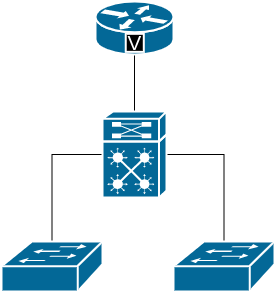
\includegraphics[width=0.3\textwidth]{virtual_switch.png}
\caption{\label{fig:vss}The connection between a VSS and a device.}
\end{figure}

\subsection{BGP}
BGP is a standardized exterior gateway protocol designed to exchange routing and reachability information among ASs on the Internet. BGP is classified as a path-vector routing protocol. BGP creates network stability by guaranteeing routers can adapt to route failures: when one path goes down, a new path is quickly found. BGP makes routing decisions based on paths, defined by rules or network policies set by network administrators.

An AS (Autonomous System) is a collection of connected IP routing prefixes under the control of one or more network operators on behalf of a single administrative entity or domain, that presents a common and clearly defined routing policy to the Internet. BGP used for routing within an AS is called iBGP (Interior Border Gateway Protocol). In contrast, the Internet application of the protocol is called eBGP (Exterior Border Gateway Protocol). Over the Internet, the chosen routing protocol is eBGP towards the service providers, with the transit AS option turned off (our locations are not transit autonomous systems). 

It is important to mention that the network administrator must not block port 179, because IP routing and connectivity must exist between BGP peers. First, they have to reach each other, and then the TCP (Transmission Control Protocol) connection on port 179 is used by BGP, sharing routing information. Although BGP seems like a routing protocol, it has its own database. For routing, the necessary routes from this database have to be in the routing table. It has two ways, but in both cases, a given route must be proved. It means, the router knows how to reach it, which gateway to use, and what the next hop is. The network administrator must not set route redistribution, because in this case, the mentioned problem exists. It is totally not recommended. The better solution is to apply automatic synchronisation. Thus, because of the network commands or a given routing protocol a given route will be in the BGP table.

This statement is true for the other direction as well. The network administrator has to use the network command for putting a route from RIB (Routing Information Base) into the BGP table, instead of using route redistribution. After the execution of the network command, the BGP process takes the new route and pushes it into the BGP table and sends it to its neighbours.

Because of the golden rule, it is not possible to force an AS to route your data differently than they would route their own data. Another AS can drop the packets without any hesitation. Therefore, the organization should make a contract with these ASs to force them to route data differently, in the best way for moucha.org. By default, in the case of BGP an AS uses the best effort for routing. There is another useful rule which is the rule of the split horizon, but it is not the case in the current topology, because all routers are edge routers and they learn routes by eBGP.

The network administrator must set a higher number for maximum hop count because this number is one by default. It means that it is working only if two routers are connected by a single cable. Furthermore, the BGP partnership happens by default when two neighbours are in different AS. According to the best network designing principles, there are four cases when it is straightforward to use BGP:
\begin{itemize}
    \item multihoming with multiaccess
    \item remote partner network
    \item influence data path towards the network
    \item exchange routes between VRFs
\end{itemize}

As shown in Figure \ref{fig:bpgs}, it is almost always advisable to use BGP in the case of multihoming. The current topology is a multihoming-single exit since all edge routers connect to the Internet in the same way. In this case, the use of BGP is considered. In this case, it can be used for load distribution (balancing). Furthermore, in this case, it is advisable to use a loopback interface on one of the routers. It is possible that a VRF (Virtual Routing and Forwarding) is used in the routers to separate the different data streams, in which case BGP supports the exchange routes between VRFs.

\begin{figure}
\centering
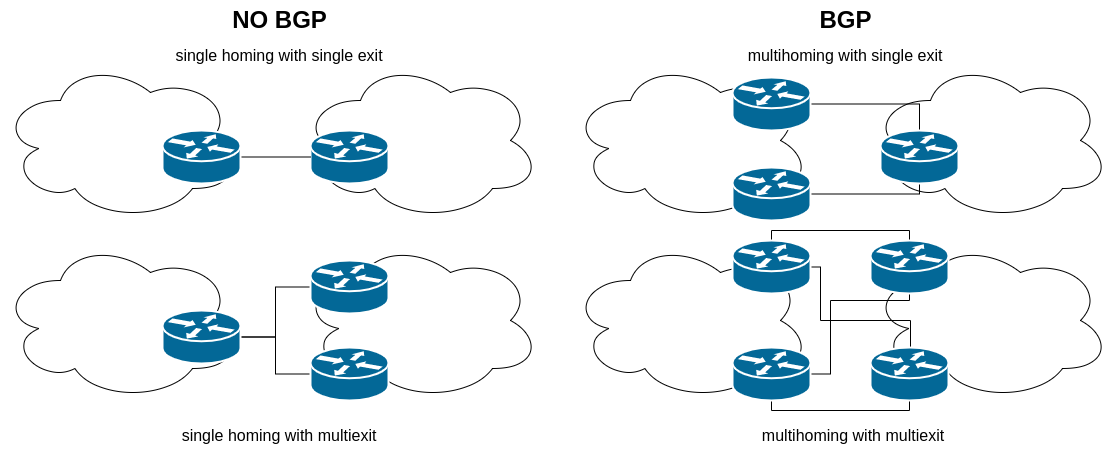
\includegraphics[width=1\textwidth]{bgps.png}
\caption{\label{fig:bpgs}Different types of connections.}
\end{figure}

With using BGP, it is pretty easy to mess up the entire routing table by inappropriate management of the tables or malicious actors. The router can think that it is connected to somebody, but it is not. A malicious actor can attack the network by sending misinformation or flooding the network with bad packets (denial-of-service attack). Moreover, one of the common BGP issues is the information exchange failure by improperly formatted or incorrect data, or the router just simply runs out of memory or storage.

BGP speed (update) is horribly slow. It is 180s because it is not necessary to poison the entire network if a cable is unplugged for a short moment. BGP is pretty static, and less dynamic because AS usually knows its partners and collaborates with them.
\subsection{VoIP and PSTN}
First and foremost, the analysation of the topology from the device's point of view shows some missing components and inefficient network design. It is high time to mention that there is no DHCP (Dynamic Host Configuration Protocol) server in the topology. This component makes the network fully functional. It gives automatically IP addresses to the devices. Without this server, static management permanently is necessary for new devices. Since DHCP allocates IP addresses for the devices and can share useful and necessary information with the devices for example default gateway and TFTP (Trivial File Transfer Protocol) server address as well. Furthermore, an important configuration is necessary on the NAS, because without this configuration the network does not have a TFTP server which can share the corresponding configuration (for example with the call manager address) with the devices.

The users cannot dial IP addresses. They dial an extension. Storage is necessary for storing telephony-related information and supporting of codec negotiation. CUCM (Cisco Unified Call Manager) deals with these tasks. There is an association between IP address and extension. CUCM remembers the devices, because of the MAC (Media Access Control) addresses. The signalling always goes through CUCM.

The last thing needed for a call is the default gateway. The problem is that there are two possible gateways for a call and the call manager cannot decide where the destination can be. The solution is to use a gatekeeper server. Gateways are registered in the gatekeeper with their usernames, passwords, certificates and so on. The network administrator has to set the priority in the possible options due to the minimization of costs. In relation to the gatekeeper, it is necessary to share information (address, details about the company, IP address of CUCM) with the DGK (Directory Gatekeeper Service), so that other organizations can access moucha.org UCM. In the current topology, a call can happen in three different ways:
    \begin{itemize}
    \item PSTN (Public Service Telephone Netwrok)
        \begin{itemize}
        \item PSTN digital
            \begin{itemize}
                    \item ISDN (Integrated Service Digital Network)
                    \item GSM (Global System for Mobile communication)
            \end{itemize}
        \item PSTN analog / POTS (Plain Old Telephone System)
        \end{itemize} 
    \item Internet (VoIP)
\end{itemize}

For communicating through PSTN some cards are necessary for the routers. Fortunately, Cisco ISR has WIC (WAN interface card) FXS (Foreign Exchange Station) card for PSTN analog and WIC ISDN PRI (Primary Rate Interface) card for PSTN digital\cite{CARDS}. Thus, these cards in the same router and one router include IPVGW (IP Voice Gateway), DVGW (Digital Voice Gateway), and AVGW (Analog Voice Gateway) functions. Moreover, if the version of the router is Release 3.11 or above then the  DSP (Digital Signalling Processor) farm services are supported. A DSP farm can be useful during codec translation and signalling as well because during codec negotiation the codec has to be common. It is not possible for devices to speak to each other with codec mismatches.

In the current topology, phones are not alone. Phones have an outcoming connection with a computer, daisy chaining. If a phone and a computer are on the same WLAN (Wireless LAN), then the computer can be sniffing on the phone line (easy configuration, huge security issue). The solution is that the phone is put on a different WLAN, using a trunk. The multi-WLAN access port solves this problem. 

Blackouts or disturbances of these institutions can lead to gaps in public safety, supply shortages, violation of data protection or other grave consequences. The Access Layer is formed by Cisco Catalyst 9500 switches with PoE (Power over Ethernet) which powers the LAPs (Lightweight Access Points), the VoIP (Voice over Internet Protocol) phones and the embedded teleconferencing systems(like cameras). This allows a single cable to provide both data connection and electrical power to devices. These devices are mission-critical devices from the organization's point of view.

The situation in the secondary location is a little bit different because there is a lack of data centres. Because of that, a Cisco SRE (Services Ready Engine)\cite{SRE} VMWare ESXi is installed inside each CR in the secondary location. It integrates all elements necessary to optimize branch-office IT infrastructure for the delivery of applications from the data centre and deployment of branch-office applications on demand. Besides that, There is CME (Call Manager Express) used in the routers. It is a call manager which uses an internal database and downloads the brief from the main location, only the necessary information to achieve SRST (Survivable Remote Site Telephony)\cite{SRST}. SRST is a CUCM call processing backup mechanism that allows Cisco IP phones to register to a Cisco router. This call manager can serve service for internal calling. this router has an FXS card and can use POTS for communicating. All other information is taken from a CUCM in a main location. A SIP (Session Initiation Protocol) trunk connects them, as shown in Figure \ref{fig:secondary_call}.

\begin{figure}
\centering
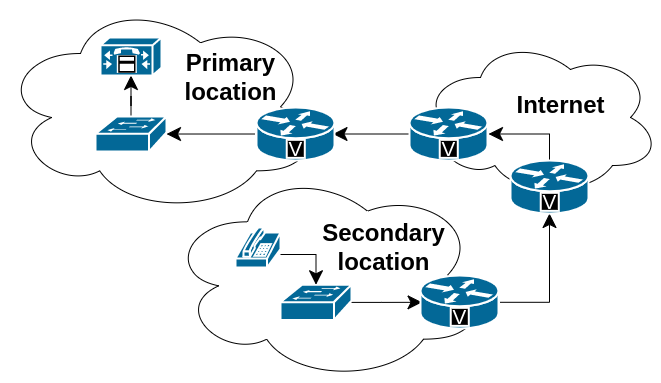
\includegraphics[width=1\textwidth]{secondary_call.png}
\caption{\label{fig:secondary_call}A call from a secondary location.}
\end{figure}

\subsection{MPLS}
The connection between the two main locations is MPLS. It is a routing technique in telecommunication networks that directs data from one node to the next based on labels rather than network addresses. It means that MPLS totally ignores the IP addresses during defining the destination. As a scalable and protocol-independent solution, MPLS assigns labels to each data packet, controlling the path the packet follows. A label defines a possible path, a unique road. By following a given label the possible destination can be easily found. It means a router sends packets along predetermined network paths and the corresponding packets take the same path every time. It reduces the time of forwarding a packet on a router. 

In MPLS, there are LSRs (Label Switch Routers) and LERs (Label Edge Routers). Since, in this topology, all routers are LER, all routers are edge routers. They sit on the edge of the organization. These routers act as a gateway between the local network and the wider area network. Whenever there is an outgoing packet to another main location, the router assigns labels to the packet. The corresponding Penultimate hop popping (PHP) technique to MPLS is when an LSR removes the label before passing the packet to the LER. The benefit is that the LSR has to do a label lookup anyway and it does not make a difference whether swap or pop the label. However, for the LER this saves one cycle of label lookup

Organizations often use this technology when they have multiple remote branch offices across the country or around the world that need access to a data centre or applications at the organization’s headquarters or another branch location. Because of that, MPLS is a good choice for communication between the two main locations.

The drawbacks of MPLS are the cost, long setup time, the difficulty of delivery globally, and lack the flexibility. MPLS is more expensive than simple Internet service. Setting up complicated dedicated paths across one or more large networks takes time. LSPs have to be manually configured by the MPLS vendor or by the organization using MPLS. The usage of MPLS makes the organization totally dependent and unflexible.

\section{New Topology}
SD-WAN provides WAN (Wide Area Network) simplification, lower costs, bandwidth efficiency and a seamless on-ramp to the cloud with significant application performance, especially for critical applications without sacrificing security and data privacy\cite{SDN_wan}. SD-Access helps organizations enable policy-based automation from the edge to the cloud. In the end, a new topology is shown with these technologies.

\subsection{SD-WAN}
SD-WAN is a WAN service with different devices and modules (V stands for Viptela, the company that developed this system):
\begin{itemize}
    \item VEDGE: sitting on the edge, IP connectivity is necessary and responsible for what is incoming into the cloud and what is outgoing out
    \item VMANAGE: GUI (Graphical User Interface) web service where it is possible to manage the whole network
    \item VSMART: decides which are the meaningful devices from the command point of view
    \item VBOND: the "glue", it sticks everything together, a public IP address is necessary
    \item CEDGE: sitting on the edge, Cisco ISR + Viptela software (from VEDGE)
\end{itemize}

There is a gap between physical and logical connectivity. In the case of SD-WAN, the physical interconnection between routers and switches is not cared. It is insignificant.

How the data is actually flowing between edges is more important. It is defined by VXLANs (Virtual Extensible LANs). GUI or direct commands make it possible to manage the system because it is an SDN, and there is an API. The communication happens by REST API (HTTP).

There are intermediate nodes between two locations that can use classic routing protocols or SD-WAN service. In both cases, the goal is to find the best path between edges.

This does not interfere with the organization's SD-WAN. If they use SD-WAN service it improves the network quality as much as possible. These new services imply a new plane among the known three, which is orchestration. Which holds the whole system together and makes various features possible. SD-WAN planes:
\begin{itemize}
    \item data
    \item management
    \item control
    \item orchestration
\end{itemize}

During the distribution of the devices, they can be distributed in different ways between different locations. Somebody physically goes there to set up the new device or the fully configured devices are shipped there. The first one is expensive. The second one is terrible from a security point of view. Fortunately, VMANAGE with encrypted communication can be used for it. Policies and templates can be created to describe the behaviour of the network. Therefore, the device can be shipped without any configuration, because after the power supply, the device will connect back to the network and get the configuration. VBOND can help with its public IP address. This is called ZTP (Zero Touch Provisioning). 

SD-WAN can automatically create a VXLAN tunnel with another router if a problem with a router is detected in the current overlay network. Application awareness with DPI (Deep Packet Inspection) monitors the traffic which passes through the edge routers. It looks inside the data packed and analyzed the traffic is whether malicious or not. It requires an extra licence, but it can be useful for example it can recognize malicious behaviour from one user which is trying to access another user's device by noticing file transfer protocol.

In SD-WAN, a VXLAN tunnel can deliver the data without dealing with IP addresses. During the delivery, there are fake IP addresses. It happens by using LISP (Locator ID Separation Protocol). The identification no longer depends on the IP address. It is a pretty similar approach to MPLS, but with better scaling. The labels have local meanings. Moreover, Routing protocols are not used and parameters are aggregated into a new parameter which is called QoE (Quality of Service). It is a subjective grade based on experience.

The last corresponding module is VANALYTICS which analysis of the current state of health and tries to predict the future by using artificial intelligence. Because of that, given parameters can be increased on time in a critical situation. 

\subsection{SD-A}
In the case of SD-WAN, any end devices are not mentioned, because their connection is provided by SD-A. SD-A also has four planes:
\begin{itemize}
    \item physical: router/switches/accesspoints/cabels, all the physical devices (underlay network)
    \item network: logical network, how those devices interconnect with each other, set of VXLAN (overlay network)
    \item control: control node, 2 devices: DNA-C + iSE
    \item management: GUI of DNA-C, GUI of iSE
\end{itemize}

DNA-C (Digital Network Architecture Center) is a hardware. It is not virtualized or a cloud service. It must be purchased. iSE (Identity Services Engine) is the identity services engine for authentication. It can be hardware or virtual machine. Besides these, there are:
\begin{itemize}
    \item FEN (Fabric Edge Node): it can also be a router or a switch which supports SDN
    \item FCN (Fabric Control Node): DNA-C + iSE
    \item FBN (Fabric Border Node): for a network or multiple networks which do not support SD-A
    \item F(V)WLC (Fabric (Virtual) Wireless LAN Controller): it is the brain of the access points
\end{itemize}

There is a CAPWAP (Control and Provisioning of Wireless Access Points) tunnel between the device and FVWLC which carries information and data. It implies horrible inefficiency. Using a wireless control card inside the switches can solve this problem because a local case remains local and it does not go through FVWLC. Another problem is the roaming. During a soft handover when the IP address of a device is not changed, an access point informs another access point about the intention. This problem is more difficult during a hard handover when the IP address of a device is changed because of the different new network, but by using the SDN approach where EID (End Device Identifier) is used it is easily solvable. IP addresses are independent of location.

Extending VLAN (Virtual LAN) beyond the switch environment is VXLAN. It creates an L2 VPN. VXLAN allows tunnelling frames from one portion of the network to a totally different portion of the network. Besides, this network does not exist, because it is an overlay network. The entire network is converted to a logical switch. This is the concept of SDN. The entire cloud becomes a switch. These switches work only for those specified data flows, nothing more, nothing less.

For SD-A, it is necessary that devices support SD-A. Fortunately, Cisco Catalyst 9600 is capable of SD-A\cite{Cat9600_sda}. Only just a software upgrade is needed for the new topology. They are programmable in one single step. Router Locator solves the location of the end device. It caches the information about the locations for 24 hours. The transportation of data in a cost-efficient way is its responsibility, but first, it must check the corresponding policy. If a policy check is not correct then the same behaviour happens like when a computer wants to communicate with a not existing IP address.  There is no change in the behaviour.

All configurations, for example, access list or firewall configuration, are easily deployable on devices. Compared to the classic network where AAA (Authentication, Authorization, and Accounting) is defined, in SD-A there are automatisation, analysis, and assurance. Automatisation means ZTP, a template for devices, no more configuration, and undoing is always possible and easy. Assurance is constantly monitoring the parameters and if some parameters are out of the predefined ranges the network will self-react and reconfigure itself. These are part of the GUI-SDA-C. The analysis is also constantly analyzing the network and logging parameters of the network.

The major difference between them is that the classic network approach is proactive. It is necessary to constantly maintain the network by doing lots of tasks. On the other hand, SDN is reactive. No enormous amount of time is wasted on maintenance. It localizes the tasks and saves lots of energy. Moreover, there are more possibilities for system analysis and anomaly detection due to the aforementioned logs and databases.

\subsection{Overview}
In the current topology,  the services are separated into two data centres, which is not efficient, but it is useful from the point of view of keeping sensitive data isolated. It is not possible to access sensitive data without authentication. In the current topology, the aforementioned spine-leaf design is applied with virtual leaves, which are virtual switches on the spine servers. The current problem is that it is inefficient from a cost perspective. Two data centres have to be maintained, but at least it is integrated into the distributed tier. It has similar functionalities to integrate into the core, but it does not apply any policies. Therefore, it is better to be in the distribution tier which is closer to the access tier. With using VLANs and IEEE 802.1x, it is possible to use only one data centre, but there is a better approach with SD-A.

\begin{figure}
\centering
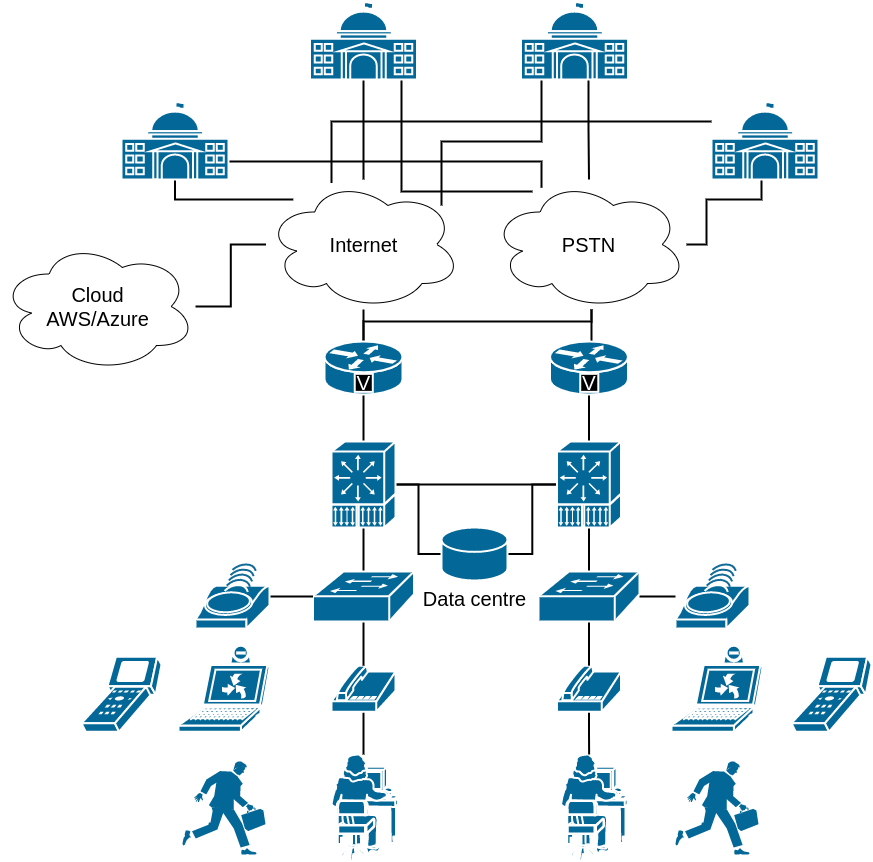
\includegraphics[width=1\textwidth]{new_top.png}
\caption{\label{fig:new_top}The created new topology.}
\end{figure}

The data centre is nothing else, just a super machine. Servers in the data centre are switches as well in the distribution tier. Lots of components and modules can be put into the data centre for example DNA-C, iSE, FVWLC, Certificate Authority, etc. Thus, the underlay network is pretty similar, but the overlay network is different. The separated traffic is not necessary anymore. All kind of macro segmentation is pointless because anyway VXLAN allows connecting with iSE and the credential information is received by the necessary module. The information flow happens only on the open VXLANs which were opened after authentication. Moreover, these tunnels are encrypted. Because of these, there is no security risk anymore to moving the data centre outside, into a cloud(AWS or Azure). There is no drawback to this change.

After these developments, only one problem remains when the local network cannot communicate with the cloud. In this case, the network cannot operate, the network is dead. The solution is that the data centre should have a local replica. The network can decide which cloud is better to communicate with based on QoE. QoE automatically tells you whether the destination data centre is local or remote.

The data in the internal data centres and in the cloud must be identical. It is the only condition in order to seamlessly working. This is not a huge problem or requirement because the network is built on SDN. It can easily establish a VXLAN from the cloud to the local data centre, with a given path transfer of the data. It synchronises all databases in real-time. The most important corresponding thing is that this is free and is part of the technology. This dynamic and flexible technology automatically makes as many tunnels as the network wants. This implies MPLS is no longer needed.

QoE is also good for reducing cabling and it avoids IXI cabling technique. The IXI redundancy cabling is not necessary anymore, because a failure is easily detectable and the network can react to it by discovering and finding a new path. Because of these, BGP is no longer needed if everything is done and defined by software.

Figure \ref{fig:new_top} shows the new network topology with using the SDN approach, with SD-WAN and SD-A. The local data centre is only for the main locations. The data centre is built in the same way as in the current topology, but it is constantly synchronizing data with the outside cloud. All mentioned services in the Eastbound and Westbound of the FTDs are deployed in the local data centres and the outside cloud. In the new topology, BGP and MPLS are not used anymore.

From the SD-WAN point of view, the routers on the edge are CEDGEs. VMANAGE, VSMART, and VBOND modules are deployed in the local data centre and the outside cloud. In the case of main location, PoE can decide which is the preferable choice. Besides these, VANALYTICS and Application awareness with DPI monitor the network traffic and provide security for the network. Thus, FirePower devices are not necessary anymore in the new topology. For these, a new license must be purchased.

From the SD-A point of view, DNA-C must be purchased and it is put into all the data centres and the outside cloud as well. This is new hardware. FVWLC is also in the data centres and the outside cloud. The switches in the access tier are the FENs of SD-A. The PTSN connection is also placed in the new topology because it is still useful and can be used in a problematic situation. All routers have the necessary cards. There is CME used in the routers in the secondary location. The configuration and transportation of a new device are developed as well. It is more easier and flexible because of ZTP.

\section{Conclusion}
They are constantly synchronising. They must run a clone. the idea is If one fails, the other one has a clone to maintain the QoE which is predefined by the organisation then everything works. The problems and shortcomings identified in section two, such as the lack of a DSP Farm or DHCP and TFTP server, significantly reduce the current network flexibility and increase the cost of the configuration. Furthermore, if we compare the current topology with the new topology, the inflexibility and security risks of the current topology are getting more incommodious. To build the new topology, the old devices can be used, but new devices, new licenses and cloud storage are required.

There are always some trade-offs, including in this case as well. A more flexible network with higher security and less maintenance time can be achieved by paying monthly large amounts of money for services. However, it is straightforward that the new topology provides a borderless enterprise which is both on the internet and on-site. Moreover, it has redundancy even though its cables are not totally redundant. It is not running BGP, and it is not looking like ASI, but the network can be made to look and behave as the organization wants.

These development suggestions make it possible for moucha.org to move from classic networking to SDN. Thus, the company has no more clear boundaries, because of dynamically establishing VXLAN tunnels.

\printbibliography

\clearpage
\glsaddall
\printglossaries

\end{document}